%\documentclass{article}
\documentclass[10pt]{article}
\usepackage{times}
%\usepackage{natbib}
%\usepackage{multicol}
\RequirePackage{natbib}
\usepackage{amsmath, amssymb, fullpage, amsthm, array,,graphicx,asa, url}
%\usepackage[dvips]{graphics}

%\usepackage{hyperref} % for hyper reference

\graphicspath{{images/}}

% \usepackage{pifont} % this package is used to print check mark \checkmark
% \linespread{1.6} % factor 1.6 = double space

%\usepackage{setspace}
%\doublespacing



\setlength{\oddsidemargin}{0in}
\setlength{\evensidemargin}{0in}
\setlength{\textwidth}{6.5in}
\setlength{\topmargin}{-0.4in}
\setlength{\textheight}{9in}
\evensidemargin 
\oddsidemargin

\newtheorem{thm}{Theorem}[section]
\newtheorem{dfn}{Definition}[section]
\newtheorem{cor}{Corollary}[thm]
\newtheorem{con}{Conjecture}[thm]
\newtheorem{lemma}[thm]{Lemma}

%\topmargin -0.10in   % when making pdf
%\textheight 9.15in  % when making pdf

\pdfminorversion=4 % as instructed by JASA file upload


\begin{document}

% Article top matter
\title{Impact of Demographics and Skills of the Observer on Visual Statistical Inference }
\author{{Mahbubul Majumder, Heike Hofmann, Dianne Cook}
\thanks{Mahbubul Majumder is a PhD student (e-mail: mahbub72@gmail.com) , Heike Hofmann is an Associate  Professor and Dianne Cook is a Professor in the Department of Statistics and Statistical Laboratory, Iowa State University, Ames, IA 50011-1210. This research is supported in part by the National Science Foundation Grant \# DMS 1007697.}}
\date{\vspace{-.5in}}
%\date{\today}  %\today is replaced with the current date
\maketitle

\begin {abstract}  
Visual Inference is dependent on the careful evaluation of the lineups by individual observers. Each individual is different in their cognitive phycology and judiciousness which can affect the power of visual inference. To estimate the power of visual inference this can be controlled by getting evaluations from multiple people from a diverse population. But the other factor that may affect the power of visual inference is the demographics and skills of the observer. In this paper we examine this in details. The simulation experiments suggest that individual skill as well as demographics are very significant for the power of visual inference. Moreover, the data shows the evidence of learning or getting skilled while sequentially evaluating multiple lineups.

{\bf Keywords: \sf statistical graphics, lineup, non-parametric test, cognitive phycology, visualization, exploratory data analysis} 
\end {abstract}

%\begin{multicols}{2}
%\twocolumn

\section{Introduction} 

The fundamental concept of visual statistical inference is introduced by \citet{buja:2009} and later these concepts are validated by \citet{majumder:2012}.

\subsection{Visual Inference} A short introduction of visual inferential procedure.
\subsection{Estimation of Power of Visual Inference} Discussion of the methods for estimating the power of visual inference \citep{majumder:2012}. 

\section{Factors Affecting the Power of Visual Inference} A brief description of the factors that may affect the power of visual inference.

\subsection{Choice of Visual Test Statistic} Discuss the effective feature of visual test statistics \citep{heike:2012}. Present some related results from \textit{Distance measure} of visual test statistics \citep{niladri:2012}.
\subsection{Question that Human Observer Faces} Discuss the importance of the question the observer needs to answer while evaluating the lineup.
\subsection{Observer Personality}
\subsection{Visual Perception of Human Eye} Discuss the results we have on eye tracking experiment \citep{zhao:2012}.
\subsection{Demographics of Observer}  Age, gender and location of the observer.
\subsection{Skills of Observer} Knowledge about statistical plot as well as education level.

\section{Simulation Experiment}

\subsection{Experiment Setup} Description of the simulation experiment giving focus on demographics and skills of experimental subjects.
\subsection{Diversity of the Experimental Subjects} Discuss why it would be important and how we accomplish this using Amazon Mechanical Turk \cite{turk} web site.

\section{Results}
\subsection{Overview of the Data}
\subsection{Learning Trend of the Observer} Since each subject is shown multiple lineups, they have a chance for self learning and do better on lineups shown later in the sequence. We examine this by fitting generalized mixed effect model presented in \cite{majumder:2012} with covariates attempt number and $p$-value of the lineup. The $p$-value of the lineup measures some sort of difficulty and including this should adjust for the difficulty level of the lineup while estimating the probability of correct responses in each attempt. Figure \ref{fig:learning_trend} shows the fitted subject wise learning pattern as well as overall learning pattern for each of the experiments. The parameter estimates od the model are shown in Table \ref{tbl:model_par}.


%\begin{table}[hbtp]
%\caption{Parameter estimates of mixed model. Estimates are highly significant with $p$-value $<$  0.0001 for all three experiment data.}
%\begin{center}
%\begin{tabular}{cr@{.}lcc}
%  \hline \hline
% &  \multicolumn{3}{c} {Fixed effect}  & Random effect\\
% \cline{2-4}
% Experiment & \multicolumn{2}{l}{Estimate}  &Std. error & Variance\\
%  \hline
%  1 & 0&39 & 0.0094 & 0.0080 \\ 
%  2 & 1&21 &  0.0197 &  0.0443 \\ 
%  3 & 0&59 (Intercept)  &   0.1668 & 1.9917\\ 
%     & 0&21 (Slope)    &  0.0511     &  0.0245\\ 
%     &-0&78 (correlation) & & \\
%   \hline
%\end{tabular}
%\end{center}
%\label{tbl:model_par}
%\end{table}




% latex table generated in R 2.15.0 by xtable 1.7-0 package
% Fri Sep  7 10:28:47 2012
\begin{table}[hbtp]
\caption{Fixed effect parameter estimates of generalized mixed model. Note that attempt is not significant for experiment 2. The continuous covariate, lineup difficulty, was measured by the $p$-value of the actual plot in the lineup.}
\begin{center}
\begin{tabular}{llrrrrl}
  \hline
& Parameters & Estimate & Std..Error & z.value & P-value  & \\ 
  \hline
\multicolumn{2}{l}{\bf{Experiment 1} } &&&& &\\
&(Intercept) & -0.30 & 0.10 & -2.89 & 0.00 & ***\\ 
 & attempt & 0.08 & 0.02 & 4.21 & 0.00 & ***\\ 
 & lineup difficulty & -11.32 & 1.01 & -11.19 & 0.00 & ***\\ 
\multicolumn{2}{l}{\bf{Experiment 2} } &&&&& \\
 & (Intercept) & 2.36 & 0.15 & 16.09 & 0.00 & ***\\ 
 & attempt & 0.01 & 0.03 & 0.35 & 0.72 \\ 
 & lineup difficulty & -55.03 & 2.20 & -25.00 & 0.00 & ***\\ 
\multicolumn{2}{l}{\bf{Experiment 3} } &&&& \\
 & (Intercept) & 0.25 & 0.16 & 1.58 & 0.11 & .\\ 
 & attempt & 0.10 & 0.03 & 3.34 & 0.00 & ***\\ 
 & lineup difficulty & 3.00 & 0.56 & 5.36 & 0.00 & ***\\ 
   \hline
\end{tabular}
\end{center}
\label{tbl:model_par}
\end{table}

% \footnote{Signif. codes: 0 �***� 0.001 �**� 0.01 �*� 0.05 �.� 0.1}


\begin{figure}[htbp] %  figure placement: here, top, bottom, or page
   \centering
   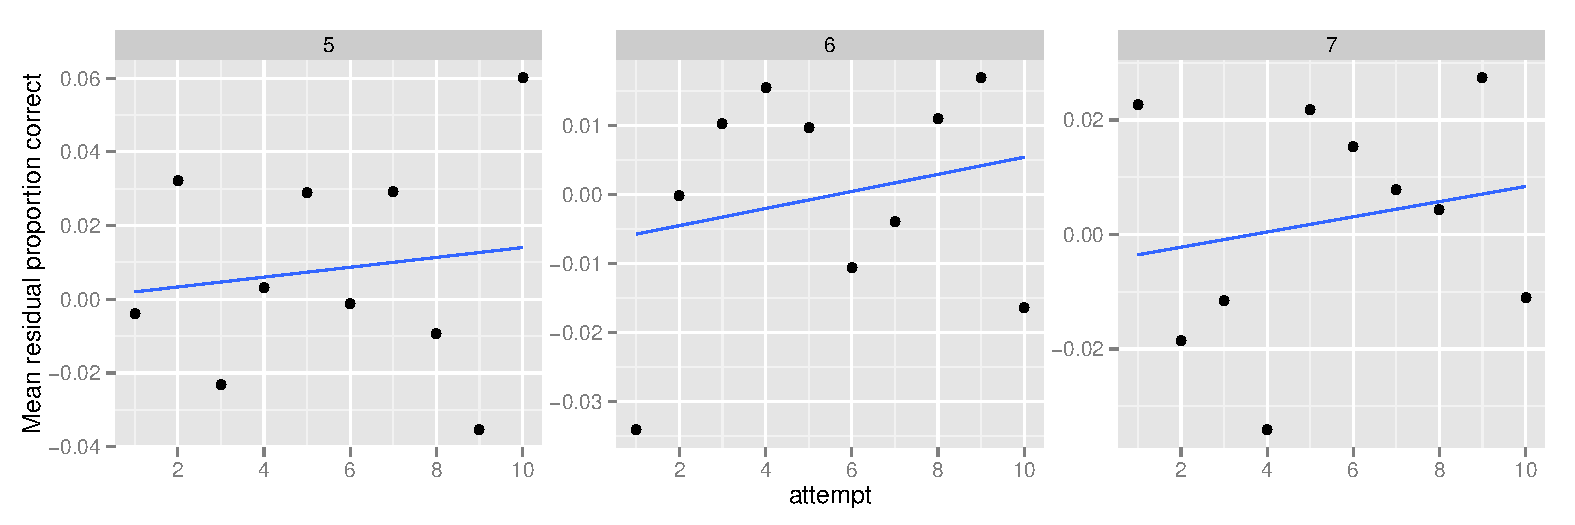
\includegraphics[width=6in]{learning_trend.pdf} 
   \caption{Probability of correct response for different attempts by each subjects for a plot with lineup difficulty ($p$-value of actual plot) = 0.05 . The overall probability increases with attempts indicating a learning trend of the observers for experiments 1 and 3. For experiment 2 the overall trend trend is not statistically significant. Subject to subject variability is seen in learning pattern.}
   \label{fig:learning_trend}
\end{figure}

\section{Conclusion}


\bibliographystyle{asa}
\bibliography{references}

\end{document}



